This chapter deals with the financial background necessary to understand the remaining of this thesis. It is targeted to readers that have already knowledge of what an investment asset is. Investments assets have many typologies and covering all would be out of scope of this work. It is sufficient to say that all of them has a price, fundamental quantity from which return and volatility are derived. Price is influenced by many factors, but in origin, how much investors have trust in that asset. This chapter deals more with \textit{how} to combine assets to form portfolio to reach investment goals. After the definition of assets and portfolio we explain diversification, a method to reduce investment risk. Then the mean-variance diagram is introduced, a way to visualize the different strategies for a portfolio construction. Subsequently, we cover different popular asset allocation methods, as this thesis create a new one of them in the later chapters.

\section{Asset return}
\label{s:asset_return}

An investment instrument that can be bough and sold is often called an \textbf{asset}.
Typical examples of assets are stocks, bonds, ETFs and futures.
An asset sold in a market has an \textbf{opening price}, the price of the asset when the market opens, and a \textbf{closing price}, the price of the asset when the market closes.
There are two important definitions to give: \textbf{total return} of an asset and \textbf{rate of return} of an asset, respectively indicated usually with $R$ for the former and $r$ for the latter. 
$$ \text{total return} = R = \frac{\text{closing price}}{\text{opening price}} $$
$$ \text{rate of return} = r = \frac{\text{closing price - opening price}}{\text{closing price}} $$
The two notions are related by:
$$ R = 1 + r $$
Frequently the shorter expression \textit{return} means the rate of return.
Because of after-hours trading, close price of day $t$ and opening price of day $t+1$ can differ.

A \textbf{cumulative return} on an investment is the total amount gained or lost by the investment throughout time, regardless of the length of time involved.
Given a sequence of rate of returns $r_i$ for $i=1,...,n$ their cumulative return is defined as
$$ C_r = \left( \prod_{i=1}^n 1+r_i \right) - 1 $$

\hfill \break

\textbf{Short selling} or \textbf{shorting} is a trading or investing technique that looks for a profit on a stock's or other security's price declining. 
To do this, an asset is borrowed by someone who owns it, such a brokerage firm. The borrowed asset is then sold to someone else, receiving an amount $X_0$. At a later date, you repay the loan by purchasing the same asset for an amount $X_1$ and return the asset to your lender. If the amount $X_1$ is lower than the original amount $X_0$, a profit of $X_0 - X_1$ is made. Therefore, short selling is profitable if the asset price declines. 
\hfill \break

Many investors regard short selling as extremely risky, if not dangerous.
The reason for this is because there is no limit to the amount of money that can be lost.
If the asset value increases, the loss is $X_1 - X_0$, since $X_1$ can increase arbitrary, so can the loss. For this reason short selling is prohibited within certain financial institutions and it purposely avoided as a policy by many individuals and institutions. In a long position, the opposite of short selling, the loss is limited by the amount invested. If we buy at price $X_0$ and sell at price $X_1$, the worst that can happen is that $X_1=0$ with a loss $L = X_0$, that would mean we lost (only) all the money we invested.
Short selling is not prohibited everywhere, and there is a significant amount of short selling of stock market assets. 
Let us determine the return associated with short selling. We receive $X_0$ initially and pay $X_1$ later, so to expenditure is $-X_0$ and the final reception is $-X_1$ and therefore return is:
$$R = \frac{-X_1}{-X_0} = \frac{X_1}{X_0}$$

The minus signs cancel out, so we obtain the same expression as using long positions. As a result, the return value $R$ applies algebraically to both long and short positions.

\

\textbf{Leverage} is when we use borrowed capital to increase the potential return of an investment. The result is to multiply the potential returns from an investment. At the same time, leverage will also multiply the potential  loss in case the investment does not succeed. 
Leverage always have a multiplier, called \textit{leverage multiplier}, that we are going now to indicate with $m$. Let us suppose we buy an asset daily leveraged at price $X_0$ and multiplier $m$, what we are actually doing is borrowing $(m-1)X_0$ capital to buy $m X_0$ amount of that asset. At the end of the day it will be sold for price $m X_1$ but our initial expenditure was only $X_0$ with an actual total return of:
$$ \text{leveraged total return} = m \frac{X_1}{X_0} $$

The borrowed capital has then to be lend back but still as a result, our return is multiplied by factor $m$ increasing both the eventual profit or loss.

\section{Portfolios}
\label{s:portfolios}

An investment portfolio is a collection of financial investments, also called assets. In some literature portfolios are also called \textit{master assets}. 

Let us suppose we have $n$ available assets. We form the portfolio by investing a specific amount in each asset. We indicate the amount invested in asset $i$ for $i=1,2,...,n$ as $X_{0i}$ such that $\sum_{i=1}^n X_{0i} = X_0$.
If we are allowed to sell and asset short, then some of the $X_{0i}$'s can be negative, otherwise we restring $X_{0i}^s$ to be non negative.
The amounts invested can be expressed as fractions of the total investment. Therefore we write:
$$ X_{0i} = w_i X_0, \: i = 1, 2, ..., n$$
where $w_i$ is the \textbf{weight} or fraction of asset $i$ in the portfolio. Clearly:
$$ \sum_{i=1}^n w_i = 1$$
and some $w_i$'s can be negative is short selling is allowed.
Let $R_i$ denote the total return of asset $i$. Then the amount of money generated at the end of the period by the $i$th asset is $R_iX_{0i} = R_i w_i X_0$. The total amount received by this portfolio at the end of the period is therefore $\sum_{i=1}^n R_i w_i X_0$. As a result we find that the overall total return of the portfolio is the weighted sum of the returns of its components:

$$ R = \frac{\sum_{i=1}^{n} R_i w_i X_0}{X_0} = \sum_{i=1}^n w_i R_i $$

Equivalently, since $\sum_{i=1}^n w_i = 1$, we have:
$r=\sum_{i=1}^n w_i r_i$

\section{Asset volatility}
\label{s:asset_volatility}

Since the money obtained when selling an asset is uncertain at the time of purchase the return is unknown and random. Therefore it can be described in probability theory. Many concept of probability are used in finance but here we will introduce only variance.

\hfill \break

We use the notation $\EX$ to indicate the expected value of a random variable $x$. For convenience $E(x)$ is often denoted by $\bar{x}$. Also the terms \textbf{mean} or \textbf{mean value} are often used for the expected value.

\hfill \break

The expected value of a random variable provides a useful summary of the probabilistic nature of the variable. However, typically one wants, in addition, to have a measure of the degree of possible deviation from the mean. One such measure is the \textbf{variance}.
Given a random variable $y$ with expected value $\bar{y}$, the quantity $y-\bar{y}$ is itself random, but has an expected value of zero. This is because $\EX(y-\bar{y})=\EX(y)-\EX(\bar{y})=\bar{y}-\bar{y}=0$. The quantity $(y-\bar{y})^2$ is always non negative and is large when $y$ deviates greatly from $\bar{y}$ and small when it is near $\bar{y}$. The expected value of this squared variable $(y-\bar{y})^2$ is useful measure of how much $y$ tends to vary from its expected value.
In general, for any random variable $y$ the variance of $y$ is defined as:
$$ var(y) = \EX[(y-\bar{y})^2)]$$

In mathematical expressions, variance is represented by the symbol $\sigma^2$. Therefore we write $\sigma^2_y = var(y)$ or if $y$ can be deduced by context, we simply write $\sigma^2=var(y)$.

\hfill \break

We frequently use the square root of the variance, denoted by $\sigma$ and called the \textbf{standard deviation}. It has the same units as the quantity $y$ and is another measure of how much the variable is likely to deviate from its expected value. Formally:

$$ \sigma_y = \sqrt{\EX[(y-\bar{y})^2]}$$

It is good to know, as it is useful in computations that:
\begin{equation}
    \label{eq:variance_conventient}
    \begin{split}
        var(x) & = \EX[(x-\bar{x})^2] \\
        & = \EX(x^2) - 2\EX(x)\bar{x} + \bar{x}^2 \\
        & = \EX(x^2) - \bar{x}^2
    \end{split}
\end{equation}

In finance, the term \textbf{volatility} is often used either to indicate asset variance or asset standard deviation.

\section{Portfolio covariance}
\label{s:portfolio_covariance}

When considering two or more random variables, as assets returns in a portfolio, their mutual dependence can be summarized conveniently by their \textbf{covariance}.

Let $x_1$ and $x_2$ be two asset returns with expected returns $\bar{x_1}$ and $\bar{x_2}$. The covariance of these assets is defined as:
$$ cov(x_1,x_2) = \EX[(x_1-\bar{x_1})(x_2-\bar{x_2})] $$

The covariance of two assets $x$ and $y$ is frequently denoted by $\sigma_{xy}$.
Consequently, for assets $x_1$ and $x_2$ we write $cov(x_1,x_2)=\sigma_{x_1,x_2}$ or alternatively, $cov(x_1,x_2)=\sigma_{12}$. Note that, by symmetry, $\sigma_{12}=\sigma_{21}$
Analogous to equation \ref{eq:variance_conventient} there is an alternative shorted formula for covariance that is easily derived:
$$cov(x_1,x_2)=\EX(x_1 x_2)-\bar{x_1} \bar{x_2}$$

This is useful in computations.
If two assets $x_1$ and $x_2$ have the property that $\sigma_{12}=0$, then they are said to be \textbf{uncorrelated}. Beware that if two assets are uncorrelated it does not imply that they are independent, the situation where knowledge of the return of one asset gives no information about the other. Correlation measure linear association but if the two assets are related in other non-linear ways correlation could not distinguish from independent case.

A portfolio can be composed of different assets with different return-risk ratio characteristics. An adequate balance between this can allow the investor to fit its preferences.


\section{Diversification}
\label{section:diversification}

We now determine the variance of the rate of return of a portfolio.
We denote the variance of the return of asset $i$ by $\sigma^2_i$, the variance of the rate of return of the portfolio by $\sigma^2$, and the covariance of the return of asset $i$ with asset $j$ by $\sigma^2_{ij}$:
\begin{equation}
    \begin{split}
        \sigma^2 & = \EX[(r - \bar{r})^2] \\
        & = \EX \left[ \left( \sum_{i=1}^n w_i r_i - \sum_{i=1}^n w_i \bar{r_i} \right) ^2 \right] \\
        & = \EX \left[ \left( \sum_{i=1}^n w_i(r_i - \bar{r_i}) \right) \left(\sum_{j=1}^n w_j (r_j - \bar{r_j}) \right) \right] \\
        & = \EX \left[ \sum_{i,j=1}^n w_i w_j (r_i - \bar{r_i} ) ( r_j - \bar{r_j}) \right] \\
        & = \sum_{i,j=1}^n w_i w_j \sigma_{ij}
    \end{split}
\end{equation}

This important result shows how the variance of a portfolio return can be calculated easily from the covariances of the pairs of asset returns and the asset weights used in the portfolio.

\hfill \break

Portfolio with only a few assets may be subject to a high degree of risk, represented by a relatively large variance. As a general rule, the variance of the return of a portfolio can be reduced by including additional assets in the portfolio, a process referred to as \textbf{diversification}.


This can be shown by using the following formulas. Let us suppose an example with $n$ assets, all of which are mutually uncorrelated, that means each asset is uncorrelated with any other asset in the group. Let us suppose also that the rate of return of each asset has mean $m$ and variance $\sigma^2$. A portfolio is built by taking an equal portion of the $n$ assets, that means $w_i = \frac{1}{n} \forall i$. The total rate of return of this portfolio is then:
$$r=\frac{1}{n}\sum_{i=1}^n r_i$$

But since each asset has mean rate of return $m$ also the mean value of $r$ is independent of $n$.

The variance of $r$ is:
$$\sigma(r)=\frac{1}{n^2} \sum^n_{i=1} \sigma^2 = \frac{\sigma^2}{n}$$

\begin{figure}
    \centering
    \subfloat[\centering Uncorrelated assets $\sigma^2 = 0.07$]{{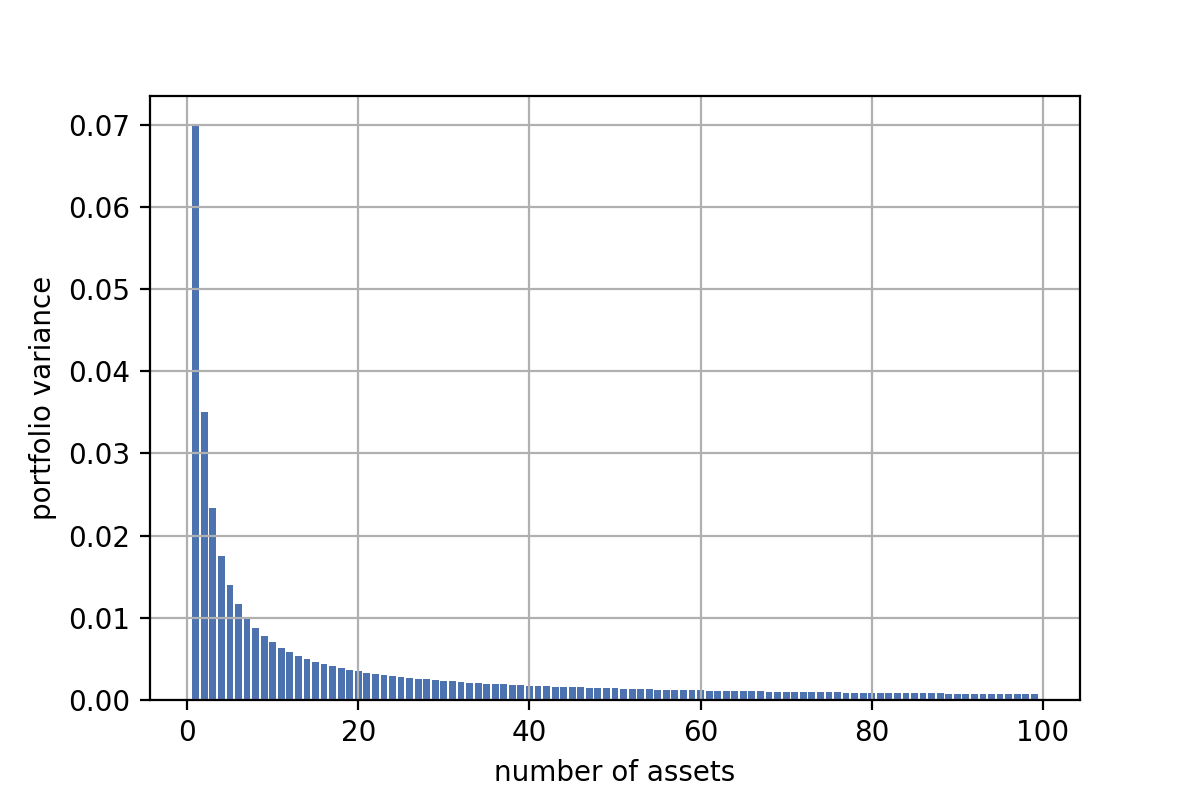
\includegraphics[width=0.7\textwidth]{cap2/port_varia_n_assets.png} }}%
    \qquad
    \subfloat[\centering Correlated assets $\sigma^2 = 0.07$ \break $cov(r_i,r_j)=\frac{1}{10}\sigma^2$]{{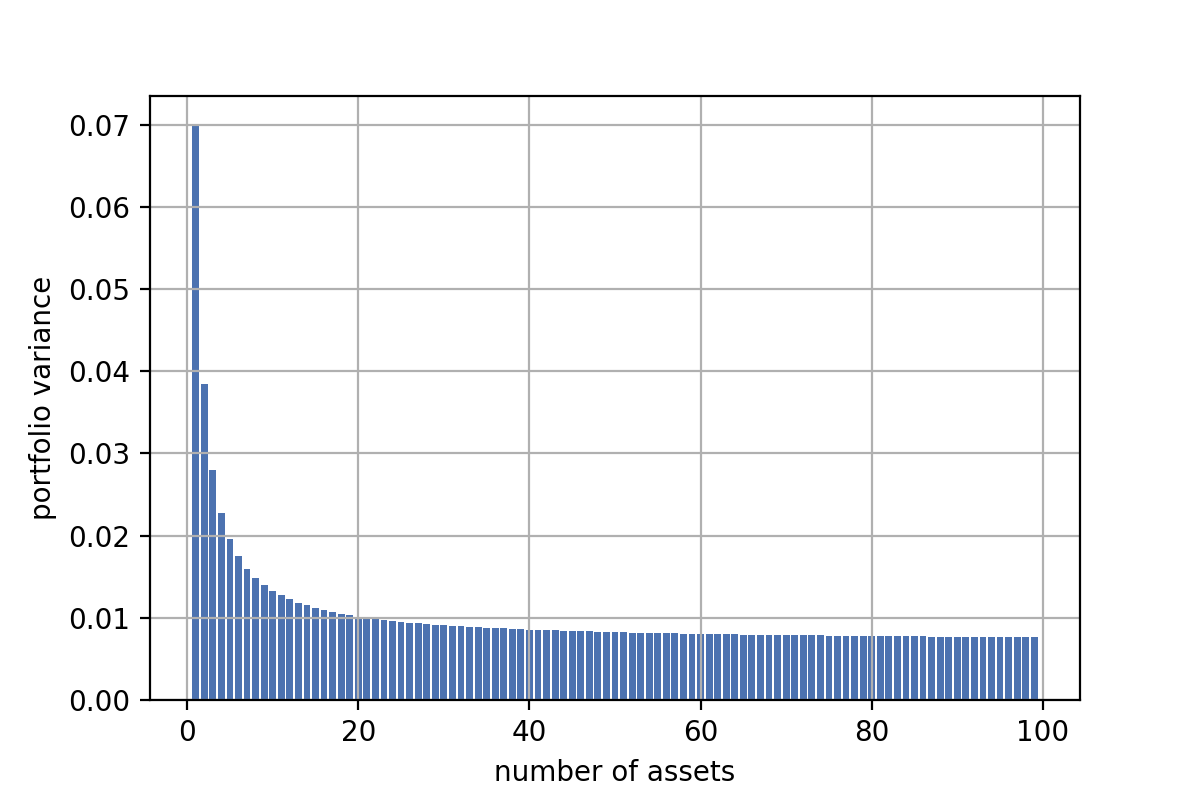
\includegraphics[width=0.7\textwidth]{cap2/port_varia_n_assets_corr.png} }}%
    \caption[Effects of diversification]{\textbf{Effects of diversification} If assets are uncorrelated variance of portfolio rapidly decrease and tends to zero by increasing number of assets. If assets are correlated there is a lower limit to variance.}
    \label{fig:portfolio_variance_assets}
\end{figure}

The variance decrease rapidly as $n$ increases, as shown in figure \ref{fig:portfolio_variance_assets}.

This is possible because we assumed that the individual returns are uncorrelated. If the asset are uncorrelated, then the variance limit to is zero:
$$ \lim_{n \rightarrow \infty} \frac{\sigma^2}{n} = 0 $$ If the assets were even partially correlated, then by adding more assets the variance would decrease slower. 

We now prove this. Let us suppose that each asset has a rate of return with mean $m$ and variance $\sigma^2$, but now each return pair is correlated by a factor $t$ and has then covariance $cov(r_i,r_j)=t \sigma^2$ for $i \neq j$. The portfolio is formed by equal portions of $n$ of these assets. In this case:

\begin{equation}
\begin{split}
var(r) & = \EX \left[ \sum_{i=1}^n \frac{1}{n}(r_i - \bar{r}) \right]^2 \\
& = \frac{1}{n^2} \EX \left\{ \left[ \sum_{i=1}^n (r_i - \bar{r}) \right] \left[ \sum_{j=1}^n (r_j - \bar{r}) \right] \right\} \\
& = \frac{1}{n^2} \sum_{i,j} \sigma_{i j} = \frac{1}{n^2} \left( \sum_{i=j} \sigma_{i j} + \sum_{i \neq j} \sigma_{i j} \right) \\
& = \frac{1}{n^2}[n \sigma^2 + t(n^2-n) \sigma^2 ] \\
& = \frac{\sigma^2}{n} + t \sigma^2 ( 1 - \frac{1}{n}) \\
& = \frac{\sigma^2(1-t)}{n} + t \sigma^2 
\end{split}
\end{equation}

This results is shown in figure \ref{fig:portfolio_variance_assets}(b). In this case it is impossible to reduce the variance below $t \sigma^2$, no matter how large is $n$
$$ \lim_{n \rightarrow \infty} \frac{\sigma^2(1-t)}{n} + t \sigma^2 = t \sigma ^2 $$


\hfill \break

In the previous analysis we assumed that the expected retun of all assets are equal. This is not, in general, the case. Diversification may reduce the overall expected return while reducing the variance. Most people are averse to reducing a considerate amount of return in exchange for a little reduction in variance, so diversification is not a task that can be executed blindly. 


\section{Mean-Variance Diagram}
\label{s:mean_variance_diagram}

The random rates of return of assets can be expressed on a two-dimensional diagram, as shown in figure \ref{fig:efficient_frontier_assets} . As asset with mean rate of return $\bar{r}$ and standard deviation $\sigma$ is represented as a point in this diagram. The standard deviation is plotted on the horizontal axis, and the vertical axis is used for the mean. This diagram is known as the \textbf{mean-standard deviation diagram}, or simply $\bar{r}-\sigma$ diagram. 

\begin{figure}[h]
    \centering
    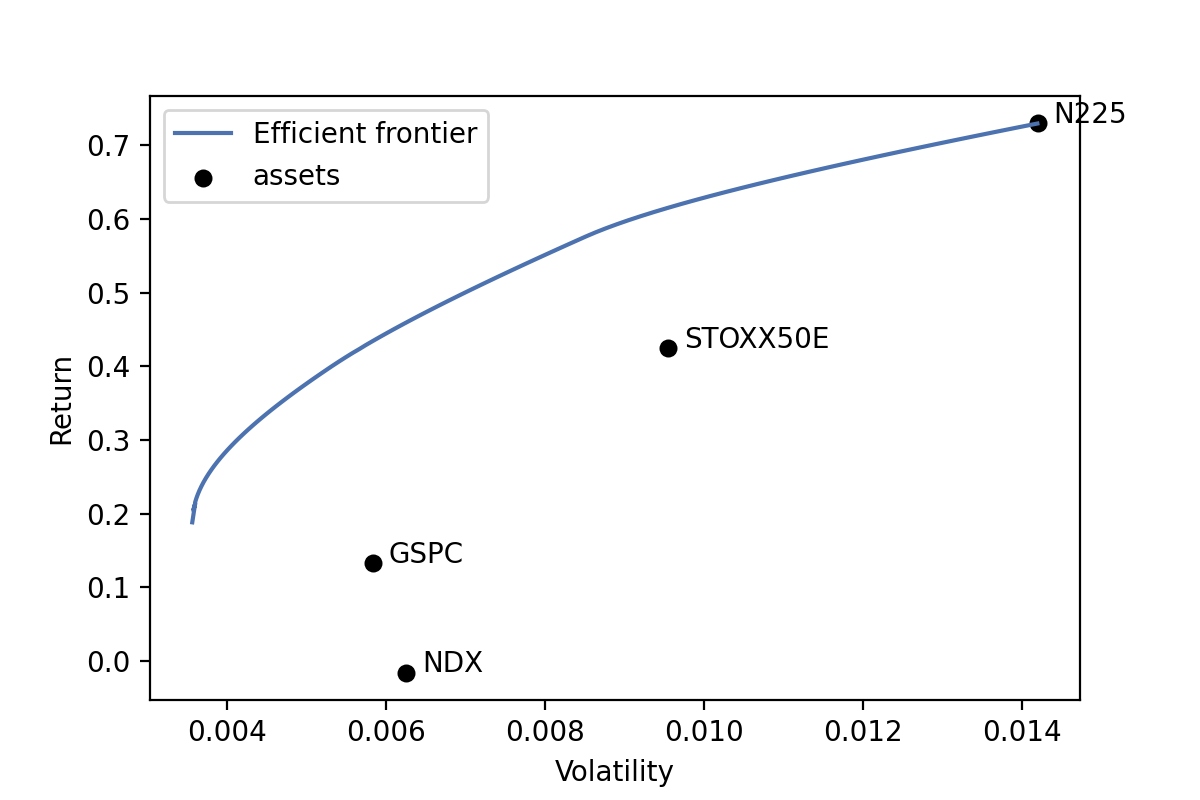
\includegraphics[width=0.7\textwidth]{Appendix/ef_assets.png}
    \caption[Mean-Variance diagram example]{Mean-Variance diagram: Points are the four different assets obtained from strategy signals and index futures used in this work, the curve is the efficient frontier of portfolios created with these assets.}
    \label{fig:efficient_frontier_assets}
\end{figure}

\hfill \break

Given $n$ assets on a mean-standard deviation 2D plot, where they are points, these assets can be combined to form a portfolio that will have a mean return and standard deviation itself, thus represented itself as a point in the diagram. 
The new portfolio mean return and standard deviation can be calculated from the assets means, variances and covariances of returns of the original assets. However, since covariances are not shown on the diagram, the exact location of the point representing the new asset cannot be determined from the location on the diagram of the original assets. There are many possibilities, depending on the covariance of the asset returns.
All these possibilities of the location of the compound portfolio in the diagram form a region, called \textbf{feasible region} or \textbf{feasible set} of points. 
With only two assets the region will be a curve, with at least three assets the region will be a two-dimensional solid region.

\hfill \break

The feasible region is convex to the left, that means that given two random points in the feasible region, the line connecting them does not cross the left boundary of the feasible region. This is because all portfolios with positive weight made from two assets lie on the left of the line connecting them. This is because the new portfolio will have always a mean return higher than the lowest mean return of the assets and a variance always lower than the highest of the assets.
If short selling is allowed, so the weights can be negative, the region will always contain the region where short selling is not allowed, as see in figure \ref{fig:random_portoflios} in the appendix.

\hfill \break

The left boundary of a feasible region is called the \textbf{minimum variance region}, since for any value of the mean rate of return, defining a horizontal line, the point will be the one with the smallest variance staying in the leftmost point of the line.
The minimum variance region has a characteristic bullet shape. There is a specific point in the minimum variance region that has a global minimum variance and is called the \textbf{minimum variance point}.
An investor that given a fixed return would always prefer the leftmost point of minimum variance is called \textbf{risk adverse investor}, and an investor that would select a point other than the one of minimum standard deviation is labelled \textbf{risk preferring investor}. We can turn the previous analysis by 90 degree and consider portfolio on a vertical line, that means portfolio with a fixed standard volatility. Investors in this case would always prefer the highest point, in others words the one with the highest return. This property of investor is called \textbf{nonsatiation}. This implies that only the upper part of the minimum variance region will be the interest of investors who are risk adverse and non satiated. The upper part of the minimum variance region is called \textbf{efficient frontier}.  

\section{Sharpe ratio}
\label{s:sharpe_ratio}

Sharpe ratio was created by Nobel Laureate William F. Sharpe and is used to help investors understand an investment's return against its risk.
The ratio is the average return earned in excess of the risk-free rate per unit of volatility or total risk.

In general, the higher the Sharpe ratio, the more attractive the risk-adjusted return of the investment. 

An investor will better isolate the profits associated with risk-taking operations by subtracting the risk-free rate from the mean return.
The risk-free rate of return is the return on a risk-free investment, i.e., the return investors would expect if they take no risk.
The risk-free rate, for example, may be the yield on a US Treasury bond. 


$$ S_r = \frac{r - r_f}{\sigma_r}$$

$r$ rate of return \\
$r_f$ Risk free return \\
$\sigma_r$ Standard deviation of returns

But the Sharpe ratio also have several limitations:
\begin{itemize}
    \item It uses standard deviation as a measure of risk. This would imply that returns are normally distributed, but financial markets shows large number of surprising drops or spikes in prices. 
    \item It focuses on volatility but not its direction. It cannot distinguish between upside and downside trends. Rare events of large positive returns should be considered beneficial, while rare large losses should be considered the opposite. The Sharpe ratio considers the two tail of the distribution the same. 
    \item As with most metrics and parameters, Sharpe ratios use historical returns and volatility. The decisions based on the ratio assume future performance will be similar to the past, that is often not true.
\end{itemize}

\hfill \break

The conversion of a short-term estimate or rate into an annual rate is known as \textbf{annualization}.
An investment with a short-term rate of return is typically annualized to get an annual rate of return, which may involve compounding or reinvestment of interest and dividends.
It is useful to annualize a rate of return in order to compare one security's performance to that of another. 
To annualize the Sharpe ratio computed on daily returns over a period of $t$ days:
$$ S_{rA} = \frac{(R - R_f) \cdot \frac{252}{t}} {\sigma_r \cdot \sqrt{252}} = S_r \cdot \frac{\sqrt{252}}{t} $$

The reason behind this is because the returns of the portfolio are diffusive, as in a Wiener process, in which volatility scales with the square-root of time. Also, in average, there are 252 trading days in a year.

\section{Post-Modern Portfolio theory}
\label{s:port_modern_portfolio_theory}

As explained above, variance is not always a the best measure of risk and Modern Portfolio theory has many critics. Post-Modern Portfolio theory (PMP) has been created \cite{rom1994post}. Markowitz itself suggested that a model based on semi-variance would be preferable, but it becomes a harder computational problem. PMP theory only use semivariance, we now give a definition of it. 
\hfill \break
The first step of calculating the semivariance is to choose a minimum acceptable return (MAR). Popular choices include zero and the risk-free rate for the year. We will use zero here. Secondly, we select only the returns that are lower or equal than the MAR. Finally the variance of this selected returns is computed.
Formally:
$$ \text{semivariance} = SV(r) = \sum_{i=1}^n (\EX[(r_i-\bar{r})^2 1_{r_i \leq 0})  $$
where $1_{r \leq 0}$ is and indicator function, i.e.
$$ 1_{r \leq 0} = \begin{cases}
    1 & if \ r \leq 0 \\
    0 & else 
\end{cases} $$


The Sortino ratio was created to address the Sharpe ratio's inability to differentiate between types of risk.
It only uses downside risk, nominally the square root of semivariance.

$$ \text{Sortino ratio} = \frac{r - r_f}{\sqrt{SV(r)}} $$

In a bull market we should seek for as much volatility as possible, only in a bear market volatility should be avoided. Individuals are more concerned with avoiding loss that seeking gains. From a practical standpoint, risk is not symmetrical. Still, in this work it is going to be used mainly Markowitz initial theory that we consider sufficient for our objectives. 



\section{Asset allocation methods}
\label{s:asset_allocation_methods}

\textbf{Asset allocation} is that part of investment science related to find an optimal balance between risk and return of a portfolio by determining or changing portfolio components weights. Rebalance of portfolio follows consideration of investor risk tolerance and investment horizon.  


\textbf{Markowitz model} is an asset allocation technique that aims to select the best asset distribution within a portfolio in order to maximize returns at a given risk level. Markowitz's work is widely known as modern portfolio theory \cite{investmentscience}. 
Markowitz problem is practically the problem of finding points on the efficient frontier.
Assuming $n$ assets each with mean (or expected) rates of return $\bar{r}_1,\bar{r}_2,...,\bar{r}_n$ and covariances $\sigma_{ij}$ for $i,j=1,2,...n$. A portfolio is defined by a set of $n$ weights $w_i$ for $i=1,2,...,n$ that sum up 1. Negative weights corresponds to short selling. To find a minimum variance portfolio, we set the mean value at some arbitrary value $\bar{r}$. Then we find the portfolio of minimum variance that has this mean. We formulate the problem as: 
\begin{align*}
    \text{minimize} \frac{1}{2} \sum_{j=1}^{n} w_i w_j \sigma_{ij}\\
    \text{subject to} \sum_{i=1}^{n} w_i \bar{r_i} = \bar{r}\\
    \sum_{i=1}^{n} w_i = 1    
\end{align*}
Once the Markowitz problem is formulated, it can be solved both analytically and numerically  to obtain a specific solution. Usually the analytical process is the most used.

Markowitz solution makes the mean and variance trade off explicit. This is useful for investors because, as seen in section \ref{section:diversification} increasing the number of assets can reduce variance, and therefore risk, but could also reduce return. Not all investors would been keen to that. Markowitz solution allows to create portfolio suitable to different demands.

\hfill \break

Predicting returns are required for mean-variance optimization and this is its primary difficulty even if the theory itself gives strong mathematical guarantees.
In practice, determining returns with a sufficient degree of accuracy is challenging and as
a result, the best we can do is often extrapolating them from historical data.

\hfill \break


There are many common algorithms for portfolio optimization and asset allocation to consider as benchmark when developing a new method, as in this case. One of the most basic ones is to give to each asset an \textbf{equal weight}, while this can be seen as very rudimental it has been observed that still can result in good performance in validation datasets \cite{PFLUG2012410} \cite{demiguel2009} \cite{duchin2009markowitz}. 

\hfill \break

A second allocation method is the \textbf{inverse volatility} method also called inverse-variance weighting. In this method every asset receive a weight proportional to the inverse of its volatility. Formally: 

$$ w_i = \frac{\frac{1}{\sigma_i}}{ \sum\limits_{j=0}^n \frac{1}{\sigma_j} } $$

\begin{figure}[h]
    \centering
    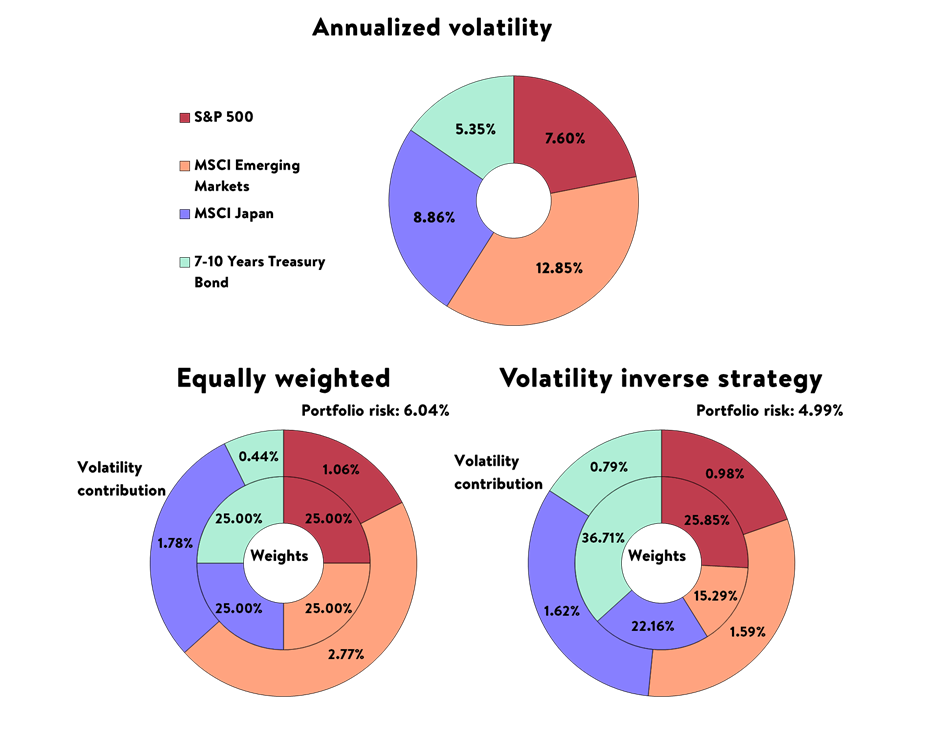
\includegraphics[width=\textwidth]{cap2/Volatility_inverse-Explanation.png}
    \caption[Inverse volatility allocation method]{Graphical explanation of inverse volatility allocation method \cite{fuertes2017}.}
    \label{volatility_inverse}
\end{figure}

\hfill \break

Another allocation method is the \textbf{risk parity} method. The objective of this method is to create a portfolio where each asset contributes equally to the portfolio overall volatility. According to the risk parity method, when asset allocations are modified (leveraged or deleveraged) to the same risk level, the risk parity portfolio can produce a higher Sharpe ratio and be more robust to market downturns than a standard portfolio \cite{teiletche2008}. 
Consider a portfolio of $n$ assets with rate of returns $r_1,...,r_n$ where the weights of the assets with rate of return $r_i$ is $w_i$. The $w_i$ form the allocation vector $w$. Let us further denote the covariance matrix of the assets by $\Sigma$. The volatility of the portfolio is then defined as the standard deviation of the random variable $w_t X$ which is:
$$ \sigma(w) = \sqrt{w' \Sigma w} $$
A risk parity portfolio can be obtained by solving the following minimization problem: 

$$ \underset{w}{\text{arg min}} \sum\limits_{i=1}^n \left( \frac{\sqrt{w^T \Sigma w}}{n} - w_i \cdot c(w)_i\right)^2 $$

Where $c(w)$ is the vector of marginal contribution to volatility of each asset $(\delta_{w_i} \sigma(w))$ and is computed as follows:
$$ c(w) = \frac{\Sigma w}{\sqrt{w' \sigma w}} $$

\begin{figure}[h]
    \centering
    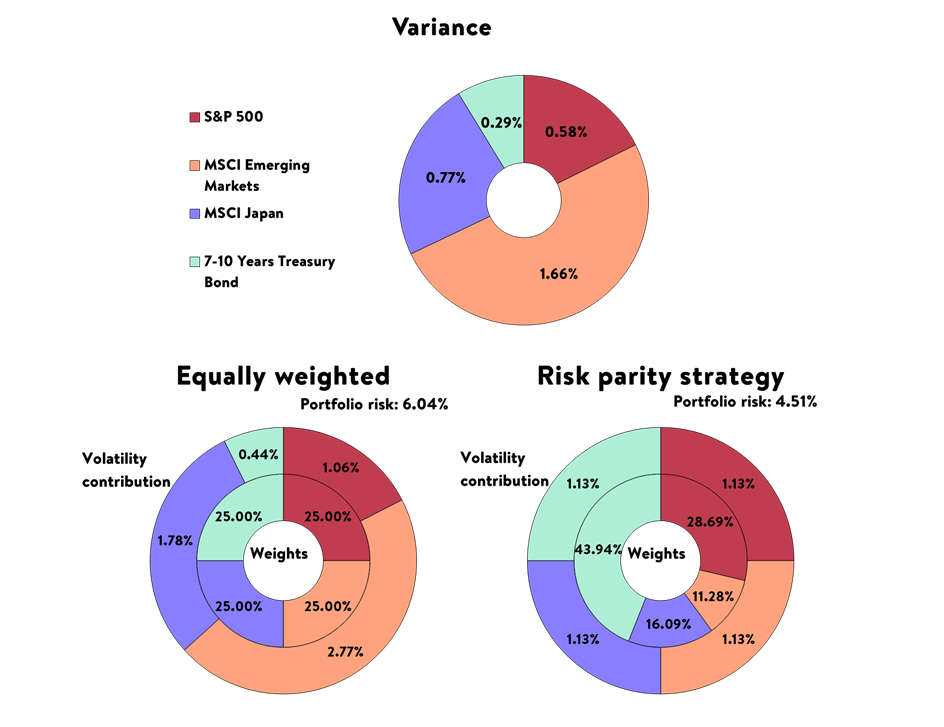
\includegraphics[width=\textwidth]{cap2/Risk-parity-Explanation.png}
    \caption[Risk parity allocation method]{Graphical explanation of risk parity allocation method \cite{fuertes2017}.}
    \label{risk_parity}
\end{figure}


\hfill \break

\section{Relative strength index}
\label{s:rsi}

Technical indicators are functions of financial quantities, generally prices or returns.  They are helpful for technical analyst to forecast movements of future prices. 

\hfill \break

One of the most used technical indicators is the \textbf{Relative Strength Index (RSI)}. The RSI is a momentum oscillator that measures price movement velocity and magnitude.
The momentum is the rate at which a price rises or falls \cite{wilder1978new}.
The RSI is most commonly utilized over a 14 day period and it can have a value from 0 to 100, with 70 and 30 being the most common high and low points.
For alternative shorter and longer outlooks, different size of time frames are used.

Each trading period is classified as up or down period. Up periods are characterized by the close being higher that the previous close. A down period is characterized by the close being lower than the previous period's close.
We calculate $U$ (Upward change) and $D$ (Downward change) as the follows for an up period:
$$U = \text{close}_{\text{now}} - \text{close}_{\text{previous}}$$
$$D=0$$
Instead, for a down period the following formula is applied:
$$U=0$$
$$D = \text{close}_{\text{previous}} - \text{close}_{\text{now}} $$

The average U and D over multiple are calculated using a $n$-period smoothed \textbf{(SMMA)}, modified (MMA) or exponential (EMA) moving average.

The \textit{relative strength factors} is the ratio of these averages:
$$RS=\frac{SMMA(U,n)}{SMMA(D,n)}$$

The relative strength factors is then normalized between 0 and 100 to obtain the relative strength index:
$$RSI = 100 - \frac{100}{1+RS}$$


Many other technical indicators exists, like Moving Average Convergence/Divergence (MACD) \cite{macd}, Bollinger bands \cite{bollinger}, Fibonacci retracement \cite{kempen2016fibonaccis}, Ichimoku cloud \cite{ichimoku}, and Average directional movement index \cite{wilder1978new}. However, due to time constraints, we were unable to test the effectiveness of using these indicators applied to the input data. The RSI was chosen as it is one of the most popular technical indicators.

\section{Volumes of trade}
\label{s:volume_of_trade}

Another financial quantities sometimes used for forecasting financial quantities are trade volumes, the total number of shares that was traded during a given period of time. While volumes have low correlation with stock returns, they have a higher correlation with volatility and can be used to forecast it. One of the earlier studies on this correlation was the work of Schwert(1989) \cite{schwert1989does} e Gallant \textit{et al.} (1992) \cite{gallant1992stock}. 

\section{Trade signal}
\label{s:trade_signal}

A trade signal is a time series indicator of suggested selling or buying of a specific security, typical with a value of $-1$ or $1$. Negative value means selling, while positive values means buying. Values outside that couple can means leverage, partial buying/selling or holding. 
Trade signal can be created by humans after a market analysis or by statistical algorithms.

\section{Market index}
\label{s:market_index}
A market index is a simulated investment portfolio that reflects a section of the financial market. Different typologies of market indexes exists: some indexes have a price that is the weighted average of its constituents price, others have a return that is the weighted average of its constituents return. Different market indices are used by investors to track market changes. 
The prices of the underlying holdings are used to calculate the index value.
There are different weighting methods for indices, here we are going only to name some: market-cap weighting, revenue-weighting, float-weighting, and fundamental-weighting.
Famous indexes are the Dow Jones Industrial Average (DJIA), S\&P 500, Nasdaq Composite Index, Eurostoxx 50, Nikkei 225.
Investors cannot invest directly in an index, so these portfolios are used mainly as benchmarks.

\section{Exchange Traded Funds and Index Futures}
\label{s:etf}
An exchange traded fund is a type of asset that have a price correlated with the value of an index, sector, commodity, or other asset, but which can be purchased or sold on a stock exchange the same way a regular stock can. 

\hfill \break

A \textbf{futures contract} is a legally binding agreement to buy or sell a certain asset at a defined price at a future date. 
Futures contract are traded on futures exchanges. 
When a futures contract is purchased, the buyer assumes the responsibility to purchase and receive the underlying asset when the contract expires.
The seller of a futures contract assumes responsibility for providing and delivering the underlying asset at the contract's expiration date. 
\textbf{Index futures} are contracts that allow a trader to purchase or sell an asset with the same price of an index today and have it resolved at a later date.
Index futures are used by traders to speculate on an index's price direction. 
